\subsection{Boundary Conditions}
The last aspect to consider in a MD simulation is the boundary conditions, understanding this as how the physical limits of the system or the spatial boundaries and external forces are modeled, and the properties of where , in reality, biologically interesting molecules are found in solvents and cells. When it comes to selecting boundary conditions, there are many options to consider with their own advantages, disadvantages, and computational cost (see Figure \ref{fig:boundary_conditions}). 
\begin{figure}[h]
    \centering
    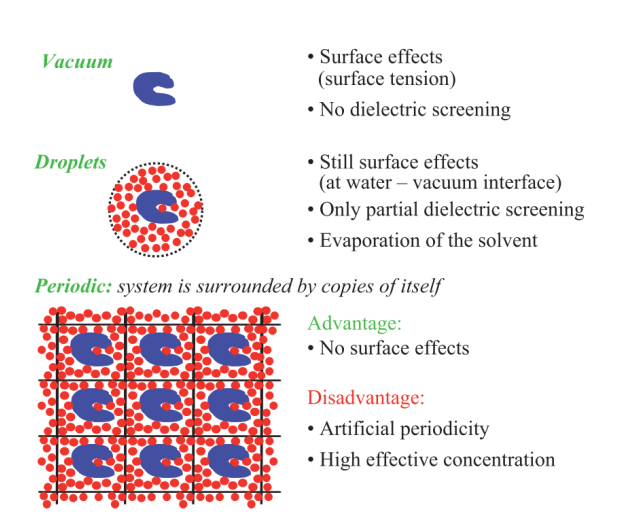
\includegraphics[scale=0.5]{Figures/Chapter2/Boundary_conditions.png}
    \caption{Three types of spatial boundary conditions used in molecular
simulation. Figure from Van Gunsten et al \cite{van2006biomolecular}}
    \label{fig:boundary_conditions}
\end{figure}
The simplest form of boundary conditions is to just simulate the molecule(s) of interest in a vacuum, however this is not representative of molecules in biological conditions and causes many problems in the surface of the molecule.
The next level of detail, and the boundary condition selected for this work because of the property that is evaluated, is when a molecule can be solvated in a droplet of solvent whit a specific geometry. However, this transfers complications from the solute-vacuum interactions to solvent-vacuum interactions, and a ``wall" must be created by fixing the position of the external solvent molecules, so that they don’t evaporate.
The method usually considered most appropriate for biological simulations is periodic boundary conditions, where the system is surrounded in all directions by copies of itself, removing surface effects and emulating bulk conditions. 